% We consider the movement of an attacker through the nodes of the attack graph as a stochastic process and interpret the state of the system as the current position of the attacker in our network. An attacker can advance to another state in the process through successful compromise of the vulnerability represented by that state only if there exists an edge in the attack graph between the attacker’s current state and the advance state.  The collection of all states in the process is the system’s state space and corresponds to the set of nodes in our attack graph. Advancing to another state is probabilistic and the success of the advance is based on the weighted score associated with that node. For example, from Figure \ref{fig:eg_ag02}, if the attacker is at Node 3, the probability that the target will be compromised is only based on the difficulty of exploiting the vulnerability on Node 1 (Trojan installation), and not on the path the attacker took to arrive at Node 3.

% Because we only need to rely on the current state of the system and not how the system arrived in that state to determine the next state, we are able to model the attack graph as a Markov Chain without loss of generality. A Markov Chain is a stochastic process that is \textit{stateless}, that is, prediction of the next system state can be made based only on the current state. This is known as the Markov Property.  

% More formally, for a stochastic process \(X = {X_t, t \geq 0}\), if the attack graph has \(n\) nodes, then the set of possible states, \(S\), for \(X\) is \(S = {s_1, s_2, \ldots, s_a, \ldots, s_n}\). The probability \(P_i,j\) that an attacker in state \(X_t\) will advance to state \(X_{t+1}\) can be given as \(P(X_{t+1} = j | X_t = i)\) with the Markov Property being satisfied as: 
% \[P(X_{t+1} = j | X_1 = x_1 , X_2 = x_2 , \ldots, X_t = i)  = P(X_{t+1} = j | X_t = i) \]
% The value \( P_{i,j}\) is known as the transition probability between two states\( s_i\) and \(s_j\). We can model the n states of the process \(X\) as an \(nxn\) matrix whose\( (i, j) \)entry is the transition probability\( P_{i,j}\). 

 

% The transition matrix
% \[
% P = \begin{bmatrix} 
%     P_{11} & \dots & P_{1n}  \\
%     \vdots & \ddots & \\
%     P_{n1} &        & P_{nn} 
%     \end{bmatrix}
% \]
% must also satisfy the conditions:  

% \[0 \leq P_{i,j} \leq 1\quad for\quad i,j \in S\]

% \[\sum_{j=1}^{n} P_{i,j} = 1\]

% That is, if a state has three outbound edges (possible choices to exploit next), the probability that any edge is followed is \(1\) since we must proceed to the attack goal after each time step, and the probability a specific edge is followed is determined by how exploitable that vulnerability is (the transition probability). This stochastic model enables us to study the system’s quantitative and qualitative properties through well-established analytic and simulation methods. Assuming the system state is given as the attacker’s current location on the attack graph (the vulnerability most recently exploited), we can model the system’s subsequent states through iteration of the stochastic process over discrete time intervals.  

 

% Attack graphs in general have the special property that the attack goal can be reached from any node in the network. This allows us to model them as an Absorbing Markov Chain using the transition matrix described above. An Absorbing Markov Chain is a Markov Chain that includes at least one absorbing state, in our case the attack goal, which can be reached from all other states, and once the absorbing state is reached (the attacker has compromised the target), no further transitions are considered.  

% \begin{figure}[H]
% \centering
% \includegraphics[width=100mm]{img/ag_2.png}
% %%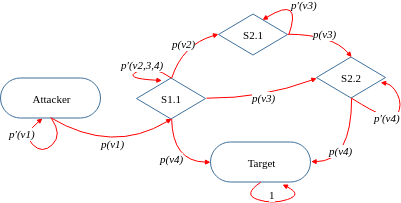
\includegraphics[width=100mm]{content/figs/eg_trans_diagram.png}
% \caption{Example Transition Diagram}
% \label{fig:ag_2}
% \end{figure} 

%     In Figure \ref{fig:ag_2} we see a  notional transition diagram. The possible states in the chain are connected by edges labeled with the probability of advancing to an adjacent state (successfully exploiting the next vulnerability.) The self-referencing edges represent the probability of an unsuccessful exploit and occur at entries \(Pi,i\) along the diagonal of the transition matrix. Note that once the system enters the ‘Target’ state no other state is reachable which we define as the absorbing state.  

 

% To create a transition matrix that conforms to our definition of an absorbing Markov chain, each outbound edge is assigned a transition probability calculated by normalizing the CVSS exploitability scores associated with all adjacent (next-step) states. That is, if we are at state \(S_i \)and the set of possible next states are given as \(Si+1 = {s1, s2, \ldots, sn}\) then we calculate the transition probability
% \[ Pij =\frac{CVSS(s_j)}{\sum_{k=1}^{n}CVSS(s_k)}; k \in S_{i+1}\]
% This normalizes the transition probabilities for all outbound states of a given state and guarantees the two conditions for a Markov transition matrix defined above will be satisfied.  

 

% The transition matrix \( P\) for the absorbing Markov chain defined above can be put into the canonical form \( P=\)
% \(\begin{bmatrix}
% Q & R \\
% 0 & I
% \end{bmatrix}\)
%   where \(Q\) is the matrix of transition probabilities for moving from a non-absorbing (transient) state to another transient state, and \(R\) is the matrix of transition probabilities for moving from a transient state to an absorbing state. In other words, we can order the rows and columns such that all transient states precede the absorbing states.  

 

% From the canonical form, \(P_k\) approaches some limiting matrix \(|P|\) as \(k\) increases, where\( |P|=\)
% \(\begin{bmatrix}
% 0 & FR \\
% 0 & I
% \end{bmatrix}\)
%   and \(F = (I-Q)-1\). This matrix \(F\) is known as the fundamental matrix for \(P\), and it allows us to derive many interesting properties from our system. For example, the\( (i, j)\) entries of \(|P|\) provide the long-term (limiting) probabilities of advancing from state \(i\) to state \(j\). Likewise, the sum of the row  entries in \(F\) determine the average number of steps it will take to reach an absorbing state from each transient state. 


% \subsection{Structural Metrics} \label{daily_tests}
% Structural metrics draw conclusions about the security properties of the attack tree through basic graph analysis techniques.  

% \textbf{Shortest Path (SP):  }

% Given an attack graph, the Shortest Path metric identifies the minimum number of nodes (vulnerabilities) an attacker would need to exploit to reach the target. Techniques for finding the shortest path in a graph are well-documented in Computer Science \cite{Dijkstra_1959}.  For the collection of paths, \(p_i\), in an attack graph \(AG\) we define the shortest path as: 

% \[SP(AG) = min(len(p1), len(p2), \ldots, len(pi), \ldots, len(pn)) \]

% The shortest path metric could be used by an attacker to identify the most direct route to a target. Another consideration is that an attacker may want to determine shortest paths as part of a minimal cut set algorithm for efficiently intercepting or degrading the target’s communications. Our findings from the SP algorithm for the three network models under test can be found in Table 5. 

% \begin{table}[H]
% \begin{tabular}{@{}lllll@{}}
% \toprule
% Structural Path Metric & Current & Transition & Final &  \\ \midrule
% Shortest Path (SP) & 4 & 3 & 3 &  \\
% Number of Paths (NP) & 6 & 3 & 1 &  \\
% Mean Path Length (MPL) & 5.33 & 4 & 3 &  \\ \bottomrule
% \end{tabular}
% \end{table}

% \textbf{Number of Paths (NP):}  

% NP is a count of the unique paths that exist on an attack graph between the attacker and the target. It is a reasonable measure of the risk exposure of the network and provides a sense of how many options an attacker would have available during a targeted attack.  
% \[NP = |p_1, p_2, \ldots, p_i, \ldots, p_n| \] 

% \textbf{Mean Path Length (MPL): }

% MPL calculates the arithmetic mean of the path lengths on the network as a way to size the average effort required to compromise a target.  

% \[MPL = \frac{\sum_{i}len(p_i)}{NP(AG)}\]
 

 

% While we can obtain some insight into the security properties of different attack graphs through direct comparison, there is not enough granularity in these structural metrics to determine the characteristic strengths or weaknesses of the underlying security posture. For example, we notice that there is a large discrepancy in the NPL measures among the three graphs; however, we can’t determine conclusively that this makes one model more susceptible to attack without knowing more about how each model’s vulnerability and exploitability relate. Effort has been made [12] to introduce statistical methods into structural metrics as a means for more reliable comparison. 
